\documentclass[a4paper,12pt]{article}

\usepackage{cmap}
\usepackage{mathtext}
\usepackage[T2A]{fontenc}
\usepackage[utf8]{inputenc}
\usepackage[english,russian]{babel}
\usepackage{listings}

\usepackage{amsmath,amsfonts,amssymb,amsthm,mathtools}
\usepackage{icomma}
\usepackage{upgreek}
\mathtoolsset{showonlyrefs=true}

\usepackage{tabto}
\usepackage{euscript}
\usepackage{mathrsfs}

\usepackage{graphicx}

\newcommand*{\hm}[1]{#1\nobreak\discretionary{}
{\hbox{$\mathsurround=0pt #1$}}{}}

\author{Kupriyanov Kirill}
\title{Data Analysis PI\\Theoretical assignment $\#6$}
\date{}

\begin{document}
\maketitle
\thispagestyle{empty}
\newpage
\section*{Task 1.}
\underline{\textit{Problem:}} Consider a linearly separable dataset and SVM
with polynomial kernel \(K(x, y) = (x^\top y + 1)^d\). Is that right, that for
any \(d > 1\) the decision boundary representation in initial feature space
will be the \textbf{error - free hyperplane} (linear decision boundary).\\
\newline
\underline{\textit{Solution:}} The decision boundary just cannot be linear if the
kernel is RBF and \(d > 1\).

For example,

\begin{figure}[h]
    \centering
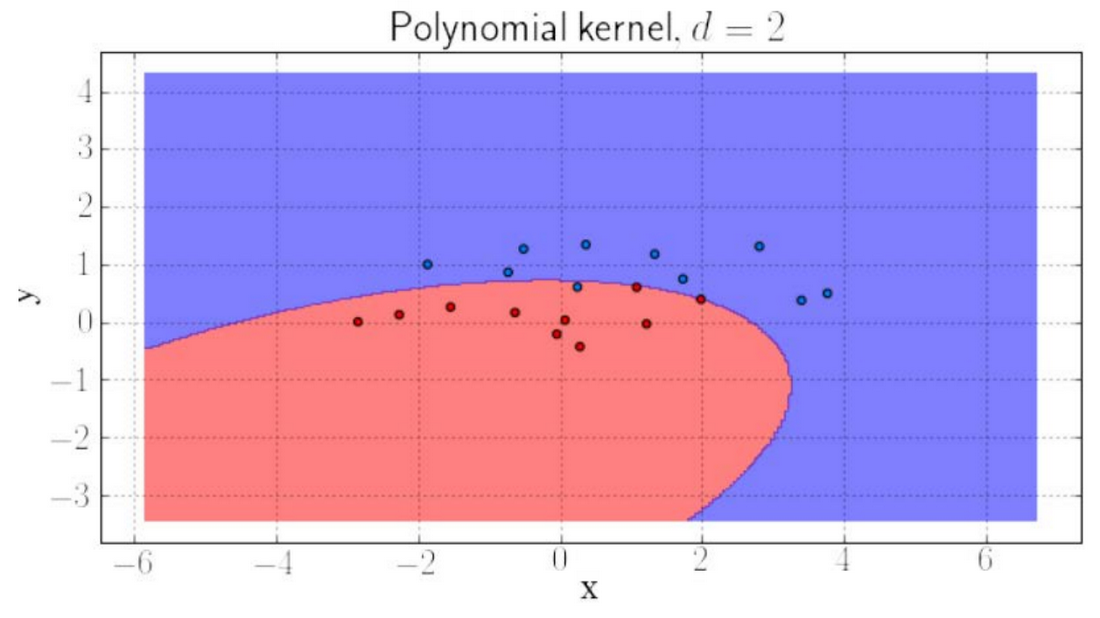
\includegraphics[width=0.7\textwidth]{example1}
\end{figure}

\newpage
\section*{Task 2.}
\underline{\textit{Problem:}} Find the computational complexity of the linear and kernel SVM \textbf{classification} procedure of a single
object (SVM is already trained).\\
\newline
\underline{\textit{Solution:}} If an input feature vector is a vector of float values, then the result is
\[
    Y = f(wx) = f\left(\sum\limits_{i=1}^{n}w_ix_i\right)
\]
Where \(w\) is a weight matrix, \(f\) - function to compute the result from dot
product.

So, the space complexity of classifying 1 object using a linear classifier
is equal to complexity of computing dot product of 2 vectors.
\[
    O(f) = O(d)
\]
,d - number of features.

SVC:
\[
    a(x) = sign(\sum\limits_{i=1}^{n} \lambda i\cdot ci\cdot xi\cdot x - b)
\]
Where:

\(x_i\) - a sample object.

\(x\) - a classidied object.

Using only those objects, for which \(\lambda \neq 0\), let's assume that \(m\) is number of objects for which \(\lambda \neq 0\). Then, the complexity will be \(O(md)\). d - number of features.

So, the linear classifier is \(O(d)\), and SVM is \(O(md)\)


\newpage
\section*{Task 3.}
\underline{\textit{Problem:}} Consider a linearly separable dataset. Write down ML loss function for logistic regression. Show that
the maximum likelihood solution for the logistic regression model is obtained by finding a vector \(w\) and
\(w_0\) with all coefficients tend to infinity.
Name a technique that can help to overcome this issue.\\
\newline
\underline{\textit{Solution:}} The binomial likelihood function looks like
follows:

\[
    L = \sum_it_i\log(p_i) + (1-t_i)\log(1-p_i)
\]
In each term in the summation only one of \(t_i\log(p_i)\) or
\((1-t_i)\log(1-p_i)\) is non-zero, with a contribution of \(p_i\) for \(t_i =
1\) and \(1-p_i\) for \(t_i = 0\).\\
\newline
To be more accurate, the following could be written:
\[
    S(\beta,x) = \frac{1}{1+\exp(-\beta x)}
\]

for the sigmoid function. There are also two limits, each approaching limit monotonically:
\begin{align}
    \lim_{\beta\rightarrow\infty} S(\beta,x) &= 0 \text{ for  }x < 0\\
    \lim_{\beta\rightarrow\infty} S(\beta,x) &= 1 \text{ for  }x > 0
\end{align}
The first limit is decreasing, the second is increasing. Each of these follows easily from the formula for \(S\).


\end{document}


% EOF

